\documentclass[11pt,a4paper]{article}

\usepackage[T1]{fontenc}
\usepackage{lmodern}
\usepackage{microtype}
\usepackage[a4paper,margin=25mm,headheight=15pt]{geometry}
\usepackage{amsmath,amssymb,amsthm,mathtools}
\usepackage{booktabs,longtable,tabularx,array}
\usepackage{graphicx}
\usepackage{xcolor}
\usepackage{enumitem}
\usepackage{listings}
\usepackage{fancyhdr}
\usepackage{caption}
\usepackage{subcaption}
\usepackage{xurl}
\usepackage[hidelinks]{hyperref}
\usepackage[nameinlink,noabbrev,capitalise]{cleveref}

\allowdisplaybreaks
\setlength{\emergencystretch}{2em}
\setlist[itemize]{topsep=4pt,itemsep=2pt,parsep=1pt}
\setlist[enumerate]{topsep=4pt,itemsep=2pt,parsep=1pt}

\definecolor{deepblue}{RGB}{27,67,112}
\definecolor{deepgreen}{RGB}{33,105,77}
\definecolor{deepred}{RGB}{137,44,44}
\definecolor{softblue}{RGB}{240,246,252}
\definecolor{softgreen}{RGB}{241,249,245}
\definecolor{softred}{RGB}{253,244,244}
\definecolor{softgray}{RGB}{246,247,249}

\hypersetup{
  pdftitle={Critical Ultradifferentiable Geometry of the Fabius--Rvachev System},
  pdfauthor={Research report prepared for the ProveIt Fabius-function corpus},
  pdfsubject={Fabius function, Rvachev up-function, Thue--Morse sequence, Denjoy--Carleman classes, Fourier decay, Lambert W, q-analogs},
  pdfkeywords={Fabius, Rvachev, Thue-Morse, Denjoy-Carleman, ultradifferentiable, Fourier, Lambert W, q-analog, Bell polynomial}
}

\pagestyle{fancy}
\fancyhf{}
\fancyhead[L]{\small Fabius--Rvachev critical regularity}
\fancyhead[R]{\small \nouppercase{\leftmark}}
\fancyfoot[C]{\thepage}

% Canonical project-wide mathematical notation.
% Canonical mathematical notation for active FabiusFunction LaTeX documents.
%
% This file is intentionally a plain TeX input rather than a LaTeX package.
% Every standalone document loads it by an explicit path relative to that
% document's directory; included fragments inherit the definitions from their
% root document.  Keep this file independent of document layout and metadata.
%
% Contract:
%   * one command has one mathematical meaning throughout the active corpus;
%   * names encode semantic roles rather than a document-local choice of letter;
%   * visually similar but differently normalized objects have different print;
%   * every command below is defined normatively in the notation catalogue.
%
% The active corpus excludes docs/archive/.  Historical sources may retain
% their original notation only inside an explicitly labelled quotation.

\makeatletter
\@ifundefined{mathbb}{%
  \PackageError{fabius-notation}{The amssymb package must be loaded first}%
    {Load amsmath and amssymb before inputting fabius-notation.tex.}%
}{}
\@ifundefined{operatorname}{%
  \PackageError{fabius-notation}{The amsmath package must be loaded first}%
    {Load amsmath before inputting fabius-notation.tex.}%
}{}
\makeatother

% Version stamp used by the catalogue and by static audits.
\newcommand{\FabiusNotationVersion}{2026-08-31}

% Number systems.  NaturalNumbers is explicitly the nonnegative convention.
\newcommand{\NaturalNumbers}{\mathbb{N}_{0}}
\newcommand{\PositiveIntegers}{\mathbb{N}_{>0}}
\newcommand{\IntegerNumbers}{\mathbb{Z}}
\newcommand{\RationalNumbers}{\mathbb{Q}}
\newcommand{\RealNumbers}{\mathbb{R}}
\newcommand{\ComplexNumbers}{\mathbb{C}}
\newcommand{\ExtendedRealNumbers}{\overline{\mathbb{R}}}

% The three principal Fabius--Rvachev functions.  Subscripts are deliberate:
% a bare F and a calligraphic F have several unrelated uses in the corpus.
\newcommand{\FabiusBounded}{F_{\mathrm{bd}}}
\newcommand{\FabiusGlobal}{F_{\mathrm{gl}}}
\newcommand{\FabiusQuantile}{Q_{F}}
\newcommand{\FabiusClampedQuantile}{Q_{F,\mathrm{cl}}}
\newcommand{\RvachevUp}{\operatorname{up}}

% Constants, elementary operators, and delimiters.
\newcommand{\EulerE}{\mathrm{e}}
\newcommand{\ImaginaryUnit}{\mathrm{i}}
\newcommand{\Differential}{\mathop{}\!\mathrm{d}}
\newcommand{\AbsoluteValue}[1]{\left\lvert #1\right\rvert}
\newcommand{\Norm}[1]{\left\lVert #1\right\rVert}
\newcommand{\Floor}[1]{\left\lfloor #1\right\rfloor}
\newcommand{\Ceiling}[1]{\left\lceil #1\right\rceil}
\newcommand{\FractionalPart}[1]{\left\{#1\right\}}
\newcommand{\PositivePart}[1]{\left(#1\right)_{+}}
\newcommand{\IndicatorOf}[1]{\mathbf{1}_{#1}}
\newcommand{\SetOf}[1]{\left\{#1\right\}}
\newcommand{\InnerProduct}[1]{\left\langle #1\right\rangle}
\newcommand{\CardinalityOf}[1]{\left\lvert #1\right\rvert}
\newcommand{\DefinitionEquals}{\mathrel{\coloneqq}}
\newcommand{\Sign}{\operatorname{sgn}}
\newcommand{\IdentityOperator}{\operatorname{id}}
\newcommand{\SpanOperator}{\operatorname{span}}
\newcommand{\TraceOperator}{\operatorname{tr}}
\newcommand{\RankOperator}{\operatorname{rank}}
\newcommand{\DiagonalOperator}{\operatorname{diag}}
\newcommand{\ResidueOperator}{\operatorname*{Res}}
\newcommand{\LeastCommonMultiple}{\operatorname{lcm}}
\newcommand{\OrderOperator}{\operatorname{ord}}
\newcommand{\PrincipalLogarithm}{\operatorname{Log}}
\newcommand{\FallingFactorial}[2]{\left(#1\right)^{\underline{#2}}}
\newcommand{\RisingFactorial}[2]{\left(#1\right)^{\overline{#2}}}

% Support, topology, convolution, and metric notation.
\newcommand{\SupportOperator}{\operatorname{supp}}
\newcommand{\SupportOf}[1]{\SupportOperator\!\left(#1\right)}
\newcommand{\TopologicalSupportOf}[1]{\operatorname{tsupp}\!\left(#1\right)}
\newcommand{\Convolution}{\mathbin{*}}
\newcommand{\MetricDistance}{\operatorname{dist}}
\newcommand{\TotalVariationDistance}{d_{\mathrm{TV}}}

% Probability.  Equality and convergence in law are not metric distance.
\newcommand{\Probability}{\mathbb{P}}
\newcommand{\Expectation}{\mathbb{E}}
\newcommand{\Variance}{\operatorname{Var}}
\newcommand{\Covariance}{\operatorname{Cov}}
\newcommand{\LawOperator}{\operatorname{Law}}
\newcommand{\LawOf}[1]{\LawOperator\!\left(#1\right)}
\newcommand{\EqualInLaw}{\mathrel{\overset{\mathrm{law}}{=}}}
\newcommand{\ConvergesInLaw}{\mathrel{\xrightarrow{\mathrm{law}}}}

% Fourier and integral transforms.  The printed labels expose normalization.
% FourierTwoPi uses exp(-2*pi*i*x*xi); FourierAngular uses exp(-i*x*omega).
\newcommand{\FourierTwoPi}[1]{\widehat{#1}_{\,2\pi}}
\newcommand{\FourierAngular}[1]{\widehat{#1}_{\,\mathrm{ang}}}
\newcommand{\LaplaceTransformSymbol}{\mathcal{L}}
\newcommand{\MellinTransformSymbol}{\mathcal{M}}
\newcommand{\LaplaceTransformOf}[1]{\LaplaceTransformSymbol\!\left[#1\right]}
\newcommand{\MellinTransformOf}[1]{\MellinTransformSymbol\!\left[#1\right]}
\newcommand{\MomentGeneratingFunction}[1]{M_{#1}}
\newcommand{\CharacteristicFunction}[1]{\varphi_{#1}}

% The two standard sinc functions must never share one symbol.
\newcommand{\SincRad}{\operatorname{sinc}_{\mathrm{rad}}}
\newcommand{\SincPi}{\operatorname{sinc}_{\pi}}

% Binary arithmetic and Thue--Morse notation.
\newcommand{\BinaryDigitSum}{\operatorname{wt}_{2}}
\newcommand{\ThueMorseSignSymbol}{\varepsilon}
\newcommand{\ThueMorseSign}[1]{\varepsilon_{#1}}
\newcommand{\PadicValuation}[1]{\nu_{#1}}
\newcommand{\TwoAdicValuation}{\nu_{2}}

% q-series notation.  Every base is an explicit argument.
\newcommand{\QPochhammer}[3]{\left(#1;#2\right)_{#3}}
\newcommand{\GaussianBinomial}[3]{%
  \genfrac{[}{]}{0pt}{}{#1}{#2}_{#3}%
}
\newcommand{\QInteger}[2]{\left[#1\right]_{#2}}

% Named special functions.
\newcommand{\Polylogarithm}{\operatorname{Li}}
\newcommand{\LambertW}{W}
\newcommand{\GammaFunction}{\Gamma}
\newcommand{\RiemannZeta}{\zeta}

% Asymptotics.  BigO and LittleO are operator tokens for existing formula
% grammar; prefer the At forms so that the limiting regime is printed.
\newcommand{\BigO}{\mathcal{O}}
\newcommand{\LittleO}{o}
\newcommand{\BigOAt}[2]{\mathcal{O}_{#2}\!\left(#1\right)}
\newcommand{\LittleOAt}[2]{o_{#2}\!\left(#1\right)}

\newtheorem{theorem}{Theorem}[section]
\newtheorem{proposition}[theorem]{Proposition}
\newtheorem{lemma}[theorem]{Lemma}
\newtheorem{corollary}[theorem]{Corollary}
\newtheorem{conjecture}[theorem]{Conjecture}
\newtheorem{problem}[theorem]{Problem}
\theoremstyle{definition}
\newtheorem{definition}[theorem]{Definition}
\newtheorem{example}[theorem]{Example}
\theoremstyle{remark}
\newtheorem{remark}[theorem]{Remark}

\newcommand{\T}{\mathbb{T}}
\newcommand{\osc}{\operatorname{osc}}
\newcommand{\id}{\operatorname{id}}
\newcommand{\comp}{\mathbin{\circ}}
\newcommand{\paren}[1]{\left(#1\right)}
\newcommand{\brak}[1]{\left[#1\right]}
\newcommand{\Roumieu}[1]{\mathcal{E}^{\{#1\}}}
\newcommand{\Beurling}[1]{\mathcal{E}^{(#1)}}
\newcommand{\DC}[1]{\mathcal{E}^{[#1]}}
\newcommand{\Wm}{W}
\newcommand{\Mm}{M}
\newcommand{\Bm}{B_C}
\newcommand{\kC}{\kappa_C}
\newcommand{\kinf}{\kappa_\infty}
\newcommand{\Lam}{\lambda}

\newcommand{\statusproved}{\textcolor{deepgreen}{\textbf{proved here}}}
\newcommand{\statussynth}{\textcolor{deepblue}{\textbf{proved synthesis}}}
\newcommand{\statusconj}{\textcolor{deepred}{\textbf{conjectural}}}

\newcommand{\resultbox}[2]{%
  \begin{center}
  \fcolorbox{#1}{softgray}{\parbox{0.92\textwidth}{\small #2}}
  \end{center}
}

\lstset{
  basicstyle=\ttfamily\small,
  breaklines=true,
  frame=single,
  columns=fullflexible,
  keepspaces=true,
  showstringspaces=false,
  keywordstyle=\bfseries,
  commentstyle=\itshape,
  numbers=left,
  numberstyle=\tiny,
  numbersep=7pt
}

\title{\textbf{Critical Ultradifferentiable Geometry of the\ Fabius--Rvachev System}\\[0.55em]
\large Local Thue--Morse universality, exact Denjoy--Carleman scales,\\
discrete Legendre duality, Lambert--$W$ saddles, and Bell-edge frontiers}
\author{Research report prepared for the ProveIt Fabius-function corpus}
\date{30 August 2026}

\begin{document}
\maketitle

\begin{abstract}
The exact derivative scale of the bounded Fabius function $\FabiusBounded$ and the Rvachev
up-function $\RvachevUp$ is
\[
  W_n=2^{n(n+1)/2}.
\]
The repository develops this scale in dyadic jet identities, endpoint asymptotics,
Fourier decay, compositional-iterate proofs, $q$-series, polynomial representations,
and several other directions.  The present report isolates a regularity-theoretic
layer that is not developed there in interval-uniform form.

First, normalized derivatives $W_n^{-1}f^{(n)}$ obey a quantitative universal law
on \emph{every} nondegenerate interval, for $f=\FabiusBounded$ or $f=\RvachevUp$.  Their pushforward
measures converge in total variation, at rate $O(2^{-n}/|J|)$, to the symmetric law
of $S\RvachevUp(Y)$, where $S$ is a Rademacher sign and $Y$ is uniform on $[-1,1]$.
Consequently every sufficiently high derivative attains both sharp extrema
$\pm W_n$ inside every interval; all local $L^p$ norms and signed moments have
universal limits.

Second, with
\[
  M_n=\frac{W_n}{n!}=\frac{2^{n(n+1)/2}}{n!},
\]
we obtain an exact local Denjoy--Carleman classification.  For any comparison
weight $N$, membership of $\FabiusBounded$ or $\RvachevUp$ in the Roumieu class $\mathcal E^{\{N\}}$
is equivalent to exponential domination of $M$ by $N$, while Beurling membership
is equivalent to strict exponential domination.  Thus $M$ is the critical local
weight on every interval.  The class is nonquasianalytic and strongly
nonquasianalytic, is stable under differentiation, composition, inversion, ordinary
differential equations, and reciprocals, but fails moderate growth drastically.
Its Fa\`a di Bruno transform is computed exactly:
\[
  M_n^{\circ}=2^nM_n.
\]
Combining this calculus with the repository's dominant-spine theorem yields a new
synthesis: every positive forward Fabius iterate and every positive inverse iterate
belongs locally to $\mathcal E^{\{M\}}$ but to no $\mathcal E^{(M)}$ on any interval.

Third, optimizing the integration-by-parts Fourier bounds gives an exact discrete
Legendre transform, including a one-periodic lattice correction.  Comparison with
the sharp sinc-product peak ray identifies the exact extra algebraic decay
$\delta=\log_2(2/\sqrt3)$.  The factorial-normalized associated function has a
different dual geometry: its saddle is governed by the lower real branch of
Lambert $W$.  These formulas extend naturally to geometric-base or $q$-deformed
weights.  Finally, exact Bell-polynomial computations through order $120$ expose a
new two-edge asymptotic hierarchy and motivate a precise $4/3$ limit conjecture.
All proved, synthesized, numerical, and conjectural assertions are explicitly
separated.
\end{abstract}

\resultbox{deepblue}{
\textbf{Status convention.}
A theorem labelled ``proved here'' is derived in this manuscript from explicitly
stated baseline identities.  A ``proved synthesis'' combines a theorem proved here
with a theorem already established in the cited ProveIt document corpus.  Numerical
observations are not promoted to theorems.  Conjectures and problems are marked as
such.  None of the new arguments is claimed to be Lean-verified.}

\begingroup
\footnotesize
\tableofcontents
\endgroup
\newpage

\section{Corpus audit, novelty boundary, and principal results}
\label{sec:audit}

\subsection{How the repository was screened}

The live documentation tree contains a primary exposition, a mathematical glossary,
a non-elementarity paper, a Lean walkthrough, a paper library, a canonical frontier
volume, a large thematic draft collection, and a frozen historical archive
\cite{ProveItDocs,ProveItArchive}.  The draft manifest describes itself as a global
inventory of every research draft and records the thematic relocations, provenance,
and overlap assessments \cite{ProveItManifest}.  The archive in turn records that
byte-identical historical copies were pruned when the live tree already preserved
them \cite{ProveItArchive}.

For the present novelty screen, the two canonical LaTeX volumes were read as the
main theorem and formula atlases, the manifest was used to traverse every active and
historical draft family, and the closest-overlap LaTeX reports were read directly.
The closest existing report is the forward-iterate manuscript
\cite{ProveItIterates}; it contains a pointwise Denjoy--Carleman interpretation but
explicitly stops short of an interval-uniform classification.  The separate Fourier
corpus already proves the sharp logarithmic-Gaussian decay and peak-ray obstruction,
so the present Fourier contribution is not a new decay theorem: it is the exact
Carleman duality and optimal comparison with the derivative envelope.

This is a corpus-wide semantic audit, not a claim of absolute publication priority.
The word ``new'' below means ``not found in the screened ProveIt LaTeX corpus in this
form.''  Frozen or absorbed duplicate documents were not treated as independent
sources of mathematical novelty.

\subsection{Overlap map}

\begin{longtable}{>{\raggedright\arraybackslash}p{0.20\textwidth}
                  >{\raggedright\arraybackslash}p{0.28\textwidth}
                  >{\raggedright\arraybackslash}p{0.42\textwidth}}
\toprule
Existing layer & Closest corpus location & Boundary respected in this report \\
\midrule
\endfirsthead
\toprule
Existing layer & Closest corpus location & Boundary respected in this report \\
\midrule
\endhead
Dyadic derivatives, Thue--Morse signs, exact cells, moments
& Primary Fabius--Rvachev exposition \cite{ProveItMain}
& Used as baseline.  The new layer is a quantitative \emph{local probability law}
on every interval, with total-variation rate and exact local extrema. \\
\addlinespace
Endpoint asymptotics and Lambert phases
& Canonical frontier volume and Lambert guide \cite{ProveItFrontier,ProveItManifest}
& Endpoint transseries are not repeated.  Lambert $W$ appears instead as the saddle
of the factorial-normalized critical weight. \\
\addlinespace
Sharp Fourier decay of the infinite sinc product
& Dedicated eight-document Fourier corpus and audits \cite{ProveItManifest}
& The sharp exponent is imported.  We derive the exact integer optimization,
periodic rounding factor, and the precise algebraic gap between Fourier decay and
derivative regularity. \\
\addlinespace
Fa\`a di Bruno defects and self-iterates
& Forward-iterate report \cite{ProveItIterates}
& Its cancellation-sensitive spine theorem is not reproved.  The new object is the
factorial-normalized weight transform $M^\circ$, computed exactly, and its use in an
interval-class synthesis for all forward and inverse iterates. \\
\addlinespace
$q$-Pochhammer, Gaussian coefficients, inverse $q$-analogs
& $q$-series monograph and several inverse/expansion reports \cite{ProveItManifest}
& No branch-inversion theory is duplicated.  We give a base-$b$/$q$ dictionary for
the critical Denjoy--Carleman weight, its associated function, and its lattice dual. \\
\addlinespace
Legendre, Lagrange, Bell--Bernoulli, Stein--Koopman, total positivity
& Representation and probability compilations \cite{ProveItManifest}
& These representations are not reproduced.  Bell polynomials enter only as the
positive majorant naturally attached to the newly identified critical weight. \\
\bottomrule
\end{longtable}

\subsection{Principal contributions}

The main claims are as follows.

\begin{enumerate}[label=\textbf{R\arabic*.},leftmargin=2.5em]
\item \statusproved: a quantitative local Thue--Morse universality theorem in total
variation, with error at most $6\,2^{1-n}/|J|$.
\item \statusproved: exact sharp extrema $\pm W_n$ on every fixed interval for all
large $n$, and universal local $L^p$ and moment limits.
\item \statusproved: an if-and-only-if local Roumieu/Beurling classification against
\emph{every} positive comparison sequence $N$.
\item \statusproved: exact weight geometry, including strong nonquasianalyticity,
failure of moderate growth, and the closed formula $M_n^\circ=2^nM_n$.
\item \statussynth: every positive forward and inverse compositional iterate has
critical local class $\mathcal E^{\{M\}}\setminus\mathcal E^{(M)}$ and quadratic
order $1/2$.
\item \statusproved: an exact discrete Legendre formula for the Fourier--Carleman
envelope, with a bounded one-periodic phase correction.
\item \statussynth: the sinc-product arithmetic contributes exactly
$\delta=\log_2(2/\sqrt3)$ powers beyond the derivative envelope, and no larger
uniform power is possible.
\item \statusproved: the standard associated function of $M$ has a
$W_{-1}$-controlled saddle and an explicit logarithmic expansion.
\item \statusproved: the weight calculus extends to geometric base $b\ge2$, or
$q=b^{-1}$, including an exact base-$b$ Fa\`a di Bruno transform.
\item \statusconj: a Bell-edge expansion whose first unremoved term is
$\frac43 n^6 4^{-n}$; exact integer arithmetic through $n=120$ supports it.
\end{enumerate}

\section{Baseline identities and notation}
\label{sec:baseline}

\subsection{Fabius, Rvachev, and Thue--Morse conventions}

Let $\FabiusBounded:[0,1]\to[0,1]$ be the bounded Fabius function and let
$\RvachevUp:\RealNumbers\to\RealNumbers$ be the compactly supported Rvachev up-function, normalized by
\[
  \SupportOperator\RvachevUp=[-1,1],\qquad \RvachevUp(0)=1,\qquad
  \int_{-1}^{1}\RvachevUp(y)\Differential y=1.
\]
On the unit interval,
\begin{equation}
  \FabiusBounded(x)=\RvachevUp(x-1),\qquad 0\le x\le1.
  \label{eq:F-up-shift}
\end{equation}
The signed Thue--Morse sequence is
\begin{equation}
  \ThueMorseSign{k}=(-1)^{s_2(k)},
  \label{eq:tm}
\end{equation}
where $s_2(k)$ is the sum of the binary digits of $k$.

Write
\begin{equation}
  T_n=\frac{n(n+1)}2,
  \qquad
  W_n=2^{T_n},
  \qquad
  h_n=2^{1-n}.
  \label{eq:weights-basic}
\end{equation}
The exact cell map is
\begin{equation}
  c_{n,k}(y)=-1+\frac{2k+1+y}{2^n},
  \qquad -1\le y\le1,
  \qquad 0\le k<2^n.
  \label{eq:cell-map}
\end{equation}
It maps $[-1,1]$ affinely onto the $k$th cell of length $h_n$ in $[-1,1]$.
The primary exposition proves the exact derivative cell identity
\begin{equation}
  \RvachevUp^{(n)}\bigl(c_{n,k}(y)\bigr)
  =W_n\ThueMorseSign{k}\RvachevUp(y).
  \label{eq:cell-identity}
\end{equation}
In particular,
\begin{equation}
  \Norm{\RvachevUp^{(n)}}_{L^\infty([-1,1])}=W_n,
  \qquad
  \RvachevUp^{(n)}\bigl(c_{n,k}(0)\bigr)=W_n\ThueMorseSign{k}.
  \label{eq:sharp-global}
\end{equation}
The shift \eqref{eq:F-up-shift} transfers these identities to $\FabiusBounded$ on $[0,1]$.
Equivalent matched-grid identities and the global signed extension of $\FabiusBounded$ are
recorded in \cite{ProveItMain,ProveItIterates}.

\subsection{A discrepancy lemma}

The local theorem rests on a particularly strong elementary feature of
Thue--Morse: every interval of indices has uniformly bounded signed discrepancy.

\begin{lemma}[Prefix and block discrepancy]
\label{lem:tm-discrepancy}
Let $P(N)=\sum_{k=0}^{N-1}\ThueMorseSign{k}$.  Then
\begin{equation}
  P(2m)=0,
  \qquad
  P(2m+1)=\ThueMorseSign{m}.
  \label{eq:prefix}
\end{equation}
Consequently, for all integers $0\le a<b$,
\begin{equation}
  \AbsoluteValue{\sum_{k=a}^{b-1}\ThueMorseSign{k}}\le2.
  \label{eq:block-discrepancy}
\end{equation}
Moreover, no three consecutive signs are equal.
\end{lemma}

\begin{proof}
The identities $\ThueMorseSign{2m}=\ThueMorseSign{m}$ and
$\ThueMorseSign{2m+1}=-\ThueMorseSign{m}$ give
\eqref{eq:prefix} by pairing.  Hence every prefix sum belongs to
$\{-1,0,1\}$, and a block sum is the difference of two prefix sums.  Finally,
each pair $(\ThueMorseSign{2m},\ThueMorseSign{2m+1})$ consists of opposite
signs, so a run of length
three is impossible.
\end{proof}

\subsection{Fourier convention}

We use
\begin{equation}
  \widehat f(\xi)=\int_{\RealNumbers}f(t)e^{-2\pi i\xi t}\Differential t.
  \label{eq:fourier-convention}
\end{equation}
For $\Phi=\widehat\RvachevUp$, the repository's product formula is
\begin{equation}
  \Phi(\xi)=\prod_{j=0}^{\infty}
  \operatorname{sinc}\!\left(\frac{\pi\xi}{2^j}\right),
  \qquad
  \operatorname{sinc}(z)=\frac{\sin z}{z}.
  \label{eq:sinc-product}
\end{equation}
The exact cell formula also gives
\begin{equation}
  \Norm{\RvachevUp^{(n)}}_{L^1(\RealNumbers)}=W_n.
  \label{eq:l1-derivative}
\end{equation}
Indeed, on every cell the absolute value is $W_n\RvachevUp(y)$ and
$\Differential x=2^{-n}\Differential y$; summing the $2^n$ cells uses $\int\RvachevUp=1$.

\section{A universal local law for high derivatives}
\label{sec:local-law}

The global derivative distribution follows immediately from the exact cells.  The
new point is that every fixed interval, however short and wherever placed, sees the
same limiting law, with an explicit total-variation error.

\subsection{The limiting probability measure}

Let $Y$ be uniform on $[-1,1]$ and let $S$ be independent with
$\mathbb P(S=1)=\mathbb P(S=-1)=1/2$.  Define the probability measure
\begin{equation}
  \mu_*=\operatorname{Law}(S\RvachevUp(Y)).
  \label{eq:mu-star}
\end{equation}
Equivalently, for every bounded Borel function $H$,
\begin{equation}
  \int H(z)\Differential\mu_*(z)
  =\frac14\int_{-1}^{1}\bigl(H(\RvachevUp(y))+H(-\RvachevUp(y))\bigr)\Differential y.
  \label{eq:mu-star-test}
\end{equation}
For a nondegenerate interval $J$ in the domain of $f$, where
$f\in\{\FabiusBounded,\RvachevUp\}$, let $\mu_{n,J}^{f}$ be the pushforward of normalized Lebesgue
measure on $J$ by $W_n^{-1}f^{(n)}$.

\begin{theorem}[Quantitative local Thue--Morse universality]
\label{thm:local-universality}
Let $f=\RvachevUp$ with $J\subseteq[-1,1]$, or $f=\FabiusBounded$ with $J\subseteq[0,1]$.
Assume $|J|>0$.  Then for every bounded Borel $H$,
\begin{equation}
 \left|
   \frac1{|J|}\int_J H\!\left(\frac{f^{(n)}(x)}{W_n}\right)\Differential x
   -\int H\Differential\mu_*
 \right|
 \le
  6\Norm{H}_\infty\frac{h_n}{|J|}.
 \label{eq:local-law-bound}
\end{equation}
Consequently,
\begin{equation}
  \TotalVariationOf{\mu_{n,J}^{f}-\mu_*}
  \le 6\frac{h_n}{|J|}
  =\frac{12}{2^n|J|},
  \label{eq:tv-bound}
\end{equation}
where
$\TotalVariationOf{\nu}
 =\sup_{\Norm{H}_\infty\le1}\AbsoluteValue{\int H\Differential\nu}$.
\end{theorem}

\begin{proof}
It suffices to prove the assertion for $\RvachevUp$, because $\FabiusBounded$ is its translate on
$[0,1]$.  Decompose $J$ into the union of all complete level-$n$ cells contained in
$J$ and at most two boundary fragments.  Let $q$ be the number of complete cells,
let their consecutive index set be $K$, and let $r=|J|-qh_n$.  Then
$0\le r\le2h_n$.

Put
\[
 A_+=\int_{-1}^{1}H(\RvachevUp(y))\Differential y,
 \qquad
 A_-=\int_{-1}^{1}H(-\RvachevUp(y))\Differential y.
\]
By \eqref{eq:cell-identity}, the contribution of the complete cells is
\[
 I_K=\frac{h_n}{2}\sum_{k\in K}A_{\ThueMorseSign{k}}.
\]
Since $q h_n\int H\Differential\mu_*=qh_n(A_++A_-)/4$, their difference is
\[
 I_K-qh_n\int H\Differential\mu_*
 =\frac{h_n}{4}\left(\sum_{k\in K}\ThueMorseSign{k}\right)(A_+-A_-).
\]
By \cref{lem:tm-discrepancy}, its absolute value is at most
$2h_n\|H\|_\infty$.

The integral on the boundary fragments has absolute value at most
$r\|H\|_\infty$, while
$r|\int H\Differential\mu_*|\le r\|H\|_\infty$.  Thus replacing the fragments by their
limiting mass costs at most $2r\|H\|_\infty\le4h_n\|H\|_\infty$.
Adding the two errors and dividing by $|J|$ proves \eqref{eq:local-law-bound}.
Taking the supremum over $\|H\|_\infty\le1$ proves \eqref{eq:tv-bound}.
\end{proof}

\begin{remark}[Strength of the convergence]
Weak convergence would follow from continuous test functions.  Here the estimate is
uniform over all bounded Borel tests, so discontinuous threshold events and local
quantiles converge at the same dyadic rate.  The only sources of error are the two
cut cells and the bounded Thue--Morse sign imbalance.
\end{remark}

\subsection{Exact local extrema and oscillation}

\begin{corollary}[Every interval eventually contains both sharp signs]
\label{cor:local-extrema}
Under the hypotheses of \cref{thm:local-universality}, if
\begin{equation}
  h_n\le\frac{|J|}{5},
  \label{eq:cell-threshold}
\end{equation}
then $J$ contains at least three complete level-$n$ cells and hence cells of both
Thue--Morse signs.  Therefore
\begin{equation}
 \max_{x\in J}f^{(n)}(x)=W_n,
 \qquad
 \min_{x\in J}f^{(n)}(x)=-W_n,
 \label{eq:local-extrema}
\end{equation}
and
\begin{equation}
  \Norm{f^{(n)}}_{L^\infty(J)}=W_n,
  \qquad
  \osc_J f^{(n)}=2W_n.
  \label{eq:local-osc}
\end{equation}
In particular these equalities hold for every sufficiently large $n$ on every fixed
nondegenerate interval.
\end{corollary}

\begin{proof}
At most two cells meeting $J$ fail to be complete, so the number $q$ of complete
cells satisfies $q\ge |J|/h_n-2\ge3$.  A consecutive block of at least three
Thue--Morse signs contains both signs by \cref{lem:tm-discrepancy}.  At the midpoint
of a positive or negative cell, \eqref{eq:cell-identity} and $\RvachevUp(0)=1$ give the
values $\pm W_n$.  The global bound \eqref{eq:sharp-global} shows that they are the
extrema.
\end{proof}

This result is much more rigid than a global supremum statement.  It says that
flatness at the endpoints does not lower the derivative class on any one-sided
neighborhood: arbitrarily high derivatives recover both global extrema at distances
of order $2^{-n}$.

\subsection{Universal local moments and \texorpdfstring{$L^p$}{Lp} norms}

\begin{corollary}[Local $L^p$ asymptotics]
\label{cor:lp}
For every $p>0$,
\begin{equation}
 \lim_{n\to\infty}
 \frac{1}{|J|W_n^p}\int_J\AbsoluteValue{f^{(n)}(x)}^p\Differential x
 =\frac12\int_{-1}^{1}\RvachevUp(y)^p\Differential y.
 \label{eq:lp-limit}
\end{equation}
For $p=1$ this becomes
\begin{equation}
  \Norm{f^{(n)}}_{L^1(J)}
  =\frac{|J|}{2}W_n+O(h_nW_n).
  \label{eq:l1-local}
\end{equation}
More generally, for every integer $m\ge0$,
\begin{equation}
 \lim_{n\to\infty}
 \frac{1}{|J|W_n^m}\int_J f^{(n)}(x)^m\Differential x
 =\begin{cases}
  0,&m\text{ odd},\\[2mm]
  \displaystyle\frac12\int_{-1}^{1}\RvachevUp(y)^m\Differential y,&m\text{ even}.
 \end{cases}
 \label{eq:signed-moment-limit}
\end{equation}
All errors are $O(h_n/|J|)$ after normalization, with constants depending only on
the bounded test function.
\end{corollary}

\begin{proof}
Apply \cref{thm:local-universality} to $H(z)=|z|^p$ and $H(z)=z^m$ on
$[-1,1]$.  For $p=1$, use $\int_{-1}^{1}\RvachevUp=1$.
\end{proof}

\begin{corollary}[Exact local quadratic derivative order]
\label{cor:local-order}
For $f=\FabiusBounded$ or $f=\RvachevUp$ and every nondegenerate interval $J$ in its domain,
\begin{equation}
 \lim_{n\to\infty}
 \frac{\log_2\Norm{f^{(n)}}_{L^\infty(J)}}{n^2}
 =\frac12.
 \label{eq:quadratic-order}
\end{equation}
\end{corollary}

\begin{proof}
By \cref{cor:local-extrema}, the numerator equals
$\log_2W_n=n(n+1)/2$ for all sufficiently large $n$.
\end{proof}

\section{The exact local Denjoy--Carleman scale}
\label{sec:dc-classification}

\subsection{Roumieu and Beurling conventions}

Let $N=(N_n)_{n\ge0}$ be any positive sequence.  On a compact interval $J$, write
$f\in\Roumieu{N}(J)$ when there exist $C,\rho>0$ such that
\begin{equation}
  \Norm{f^{(n)}}_{L^\infty(J)}
  \le C\rho^n n!N_n
  \qquad(n\ge0).
  \label{eq:roumieu-def}
\end{equation}
Write $f\in\Beurling{N}(J)$ when for every $\rho>0$ there exists $C_\rho>0$ for
which \eqref{eq:roumieu-def} holds.  These are the standard factorial-normalized
Denjoy--Carleman conventions \cite{RainerClosedSets,RainerSchindl}.

Define the critical sequence
\begin{equation}
  M_n=\frac{W_n}{n!}
  =\frac{2^{n(n+1)/2}}{n!},
  \qquad M_0=1.
  \label{eq:critical-weight}
\end{equation}

\subsection{Complete comparison theorem}

\begin{theorem}[Exact local comparison against every weight]
\label{thm:dc-classification}
Let $f=\FabiusBounded$ or $f=\RvachevUp$, and let $J$ be any nondegenerate compact interval in its
domain.  For every positive sequence $N$,
\begin{align}
  f\in\Roumieu{N}(J)
  &\iff
  \limsup_{n\to\infty}
  \left(\frac{M_n}{N_n}\right)^{1/n}<\infty,
  \label{eq:roumieu-criterion}\\
  f\in\Beurling{N}(J)
  &\iff
  \limsup_{n\to\infty}
  \left(\frac{M_n}{N_n}\right)^{1/n}=0.
  \label{eq:beurling-criterion}
\end{align}
Thus the local regularity class is independent of the position and length of $J$;
only the finite threshold after which the sharp derivative values occur depends on
$J$.
\end{theorem}

\begin{proof}
By \cref{cor:local-extrema},
\[
  \Norm{f^{(n)}}_{L^\infty(J)}=W_n=n!M_n
\]
for every sufficiently large $n$.  If \eqref{eq:roumieu-def} holds, division by
$n!N_n$ and passage to $n$th roots gives the necessity of
\eqref{eq:roumieu-criterion}.  Conversely, finite limsup means that
$M_n\le C\rho^nN_n$ for some $C,\rho$ after increasing $C$ to absorb finitely many
initial terms.

The Beurling statement is the same argument with every $\rho>0$.  A positive
sequence $a_n$ satisfies $a_n\le C_\rho\rho^n$ for every $\rho>0$ if and only if
$\limsup a_n^{1/n}=0$.
\end{proof}

\begin{corollary}[Critical Roumieu but not critical Beurling]
\label{cor:critical-class}
On every nondegenerate interval $J$,
\begin{equation}
  f\in\Roumieu{M}(J)
  \quad\text{but}\quad
  f\notin\Beurling{M}(J).
  \label{eq:critical-not-beurling}
\end{equation}
The weight $M$ is therefore exact up to ordinary exponential equivalence.
\end{corollary}

\begin{proof}
In \cref{thm:dc-classification} take $N=M$.  The comparison ratio is identically
one.
\end{proof}

\begin{corollary}[No finite Gevrey order on any interval]
\label{cor:no-gevery}
For every finite $s\ge1$, neither $\FabiusBounded$ nor $\RvachevUp$ belongs locally on any nondegenerate
interval to the Gevrey class with derivative bounds $C\rho^n(n!)^s$.
\end{corollary}

\begin{proof}
The Gevrey-$s$ sequence is $N_n=(n!)^{s-1}$.  Stirling's formula gives
\[
 \frac1n\log\left(\frac{M_n}{N_n}\right)
 =\frac{\log2}{2}n-s\log n+O(1)\longrightarrow+\infty.
\]
Thus even the Roumieu criterion fails.
\end{proof}

\begin{corollary}[Sharp transition among quadratic exponential classes]
\label{cor:quadratic-classes}
For $\alpha>0$, let $\mathcal Q_\alpha$ denote the class with derivative bound
$C\rho^n2^{\alpha n^2}$.  On every nondegenerate interval,
\begin{align}
 f\in\mathcal Q_\alpha^{\{\cdot\}}
 &\iff \alpha\ge\frac12,
 \label{eq:q-roumieu}\\
 f\in\mathcal Q_\alpha^{(\cdot)}
 &\iff \alpha>\frac12.
 \label{eq:q-beurling}
\end{align}
At $\alpha=1/2$, the residual factor $2^{n/2}$ is exactly of Roumieu exponential
type but not of Beurling type.
\end{corollary}

\begin{proof}
Use $N_n=2^{\alpha n^2}/n!$.  Then
\[
 \left(\frac{M_n}{N_n}\right)^{1/n}
 =2^{(1/2-\alpha)n+1/2}.
\]
Apply \cref{thm:dc-classification}.
\end{proof}

\subsection{A local regularity spectrum}

The theorem can be packaged as an intrinsic spectrum.  For any smooth $g$ on a
compact interval $J$, define
\begin{equation}
  \tau_J(g;M)=
  \limsup_{n\to\infty}
  \left(\frac{\Norm{g^{(n)}}_{L^\infty(J)}}{n!M_n}\right)^{1/n}.
  \label{eq:carleman-type}
\end{equation}
Then $g\in\Roumieu{M}(J)$ exactly when $\tau_J(g;M)<\infty$, and
$g\in\Beurling{M}(J)$ exactly when $\tau_J(g;M)=0$.  For the basic functions,
\begin{equation}
  \tau_J(\FabiusBounded;M)=\tau_J(\RvachevUp;M)=1.
  \label{eq:type-one}
\end{equation}
Thus every interval has the same exact Carleman type, even intervals adjacent to a
flat endpoint.

\section{Geometry of the critical weight}
\label{sec:weight-geometry}

The critical sequence is unusual: it has enough convexity for a full nonlinear
calculus and enough growth to be nonquasianalytic, yet it is far outside the
moderate-growth regime.

\subsection{Quotients, nonquasianalyticity, and derivations}

\begin{theorem}[Exact structural properties of $M$]
\label{thm:weight-properties}
The sequence \eqref{eq:critical-weight} has the following properties.
\begin{enumerate}[label=(\roman*)]
\item Its quotients are
\begin{equation}
  \mu_n:=\frac{M_n}{M_{n-1}}=\frac{2^n}{n}
  \qquad(n\ge1).
  \label{eq:quotient}
\end{equation}
Hence $M$ is logarithmically convex and $M_n^{1/n}$ is increasing.
\item It is nonquasianalytic, with exact Denjoy--Carleman sum
\begin{equation}
  \sum_{k=0}^{\infty}
  \frac{M_k}{(k+1)M_{k+1}}
  =\sum_{k=0}^{\infty}2^{-(k+1)}=1.
  \label{eq:nqa-sum}
\end{equation}
\item It is strongly nonquasianalytic.  For $k\ge1$,
\begin{equation}
  \sum_{j\ge k}\frac{M_{j-1}}{jM_j}
  =2^{1-k}
  \le2\frac{M_{k-1}}{M_k}.
  \label{eq:strong-nqa}
\end{equation}
\item It is derivation closed:
\begin{equation}
  \sup_{n\ge1}
  \left(\frac{M_{n+1}}{M_n}\right)^{1/n}<\infty,
  \qquad
  \lim_{n\to\infty}
  \left(\frac{M_{n+1}}{M_n}\right)^{1/n}=2.
  \label{eq:derivation-closed}
\end{equation}
\item It does not have moderate growth.  In fact
\begin{equation}
  \frac{M_{2n}}{M_n^2}
  =\frac{2^{n^2}}{\binom{2n}{n}}
  \ge2^{n^2-2n}.
  \label{eq:nonmoderate}
\end{equation}
\end{enumerate}
\end{theorem}

\begin{proof}
The quotient formula is immediate from $T_n-T_{n-1}=n$.  Moreover,
$\mu_{n+1}/\mu_n=2n/(n+1)\ge1$, proving log-convexity.
The remaining exact sums follow from
\[
  \frac{M_k}{(k+1)M_{k+1}}=2^{-(k+1)},
  \qquad
  \frac{M_{j-1}}{jM_j}=2^{-j}.
\]
The derivation condition follows from
$M_{n+1}/M_n=2^{n+1}/(n+1)$.  Finally,
\[
 \frac{M_{2n}}{M_n^2}
 =2^{T_{2n}-2T_n}\frac{(n!)^2}{(2n)!}
 =\frac{2^{n^2}}{\binom{2n}{n}},
\]
and $\binom{2n}{n}\le4^n$.
\end{proof}

\begin{remark}
Nonquasianalyticity is consistent with the compact support of $\RvachevUp$.  Moderate
growth, by contrast, would require a uniform exponential control of
$M_{j+k}/(M_jM_k)$; the quadratic exponent creates an unavoidable factor
$2^{jk}$, so moderate growth fails by an exponentially widening margin.
\end{remark}

\subsection{The exact Fa\`a di Bruno transform}

For a positive sequence $M$, define the Fa\`a di Bruno transform
\begin{equation}
  M_n^\circ=
  \max\left\{
    M_jM_{\alpha_1}\cdots M_{\alpha_j}:
    j\ge1,\ \alpha_i\ge1,\ \sum_{i=1}^j\alpha_i=n
  \right\},
  \qquad M_0^\circ=1.
  \label{eq:fdb-transform-def}
\end{equation}
This is the normalized weight that controls all chain-rule partitions
\cite{RainerSchindl}.

\begin{theorem}[Exact Fa\`a di Bruno envelope]
\label{thm:exact-fdb}
For the critical sequence $M_n=2^{T_n}/n!$,
\begin{equation}
  M_n^\circ=2^nM_n
  \qquad(n\ge0).
  \label{eq:exact-fdb}
\end{equation}
For $n\ge1$, the lower bound is attained by the partition
$j=n$, $\alpha_1=\cdots=\alpha_n=1$.
\end{theorem}

\begin{proof}
The indicated partition gives
$M_nM_1^n=2^nM_n$, because $M_1=2$.

For the upper bound, fix $j$ and a composition
$\alpha_1+\cdots+\alpha_j=n$.  Log-convexity implies that, for fixed sum, the
product $\prod_iM_{\alpha_i}$ is maximized when one part is as large as possible
and the others equal $1$.  Put
\[
  r=n-j+1.
\]
It suffices to estimate $M_jM_rM_1^{j-1}$.  Direct calculation gives
\begin{equation}
 \frac{M_jM_rM_1^{j-1}}{M_n}
 =2^{j-(j-1)(r-1)}\frac{n!}{j!r!}.
 \label{eq:fdb-ratio}
\end{equation}
Since $n=j+r-1$,
\begin{equation}
  \frac{n!}{j!r!}
  \le\binom{j+r-1}{r-1}
  \le(j+1)^{r-1}
  \le2^{j(r-1)}.
  \label{eq:factorial-bound}
\end{equation}
The middle inequality follows, for example, by encoding weakly increasing choices
by words on $j+1$ symbols, and the last uses $j+1\le2^j$.  Substitution into
\eqref{eq:fdb-ratio} gives
\[
 \frac{M_jM_rM_1^{j-1}}{M_n}
 \le2^{j-(j-1)(r-1)+j(r-1)}
 =2^{j+r-1}=2^n.
\]
Taking the maximum proves the result.
\end{proof}

\begin{remark}[Distinction from the iterate defect]
The iterate report \cite{ProveItIterates} studies the \emph{signed, unnormalized}
Fa\`a di Bruno expansion of $\FabiusBounded^{\comp r}$ and proves that branched partitions are
small after cancellation-sensitive normalization by $W_n$.  The present theorem
answers a different question: it computes the \emph{positive,
factorial-normalized} sequence transform that governs closure of the entire
Denjoy--Carleman class.  The two results are complementary.
\end{remark}

\subsection{Nonlinear stability}

The hypotheses in the Rainer--Schindl stability theorem are now explicit:
$M_n^{1/n}\to\infty$, derivation closure holds, and
$M_n^\circ\le2^nM_n$.  Therefore both types of the critical class possess the full
standard nonlinear calculus.

\begin{corollary}[Critical classes are stable under nonlinear operations]
\label{cor:stability}
The Roumieu and Beurling classes $\Roumieu{M}$ and $\Beurling{M}$ are stable under
composition, local inversion at points with nonzero Jacobian, solution of ordinary
differential equations, and reciprocal of nonvanishing functions.
\end{corollary}

\begin{proof}
Apply the Roumieu and Beurling equivalence theorems of Rainer and Schindl
\cite{RainerSchindl} using \cref{thm:weight-properties,thm:exact-fdb}.
\end{proof}

The coexistence of \cref{eq:nonmoderate} and \cref{cor:stability} is important:
moderate growth is sufficient for many convenient tensor-product and extension
results, but it is not necessary for the one-dimensional nonlinear operations
needed by the Fabius dynamics.

\section{Inverse Fabius function and all compositional iterates}
\label{sec:inverse-iterates}

Let $\FabiusQuantile:(0,1)\to(0,1)$ be the inverse of $\FabiusBounded$, and write
\[
  G_r=\FabiusBounded^{\comp r},
  \qquad
  H_r=\FabiusQuantile^{\comp r}
  \qquad(r\ge1).
\]

\subsection{The inverse function at the critical scale}

\begin{theorem}[Exact interior class of the inverse Fabius function]
\label{thm:inverse-class}
On every compact interval $K\Subset(0,1)$,
\begin{equation}
  \FabiusQuantile\in\Roumieu{M}(K)
  \quad\text{and}\quad
  \FabiusQuantile\notin\Beurling{M}(K).
  \label{eq:inverse-class}
\end{equation}
Consequently the inverse Fabius function is not of finite Gevrey order on any
nondegenerate interior interval.
\end{theorem}

\begin{proof}
The image $J=\FabiusQuantile(K)$ is compactly contained in $(0,1)$, where
$\FabiusBounded'>0$.
By \cref{cor:critical-class,cor:stability}, local inversion gives
$\FabiusQuantile\in\Roumieu{M}(K)$.  If
$\FabiusQuantile\in\Beurling{M}(K)$, Beurling inversion stability would
imply $\FabiusBounded\in\Beurling{M}(J)$, contradicting \cref{cor:critical-class}.
The Gevrey conclusion follows as in \cref{cor:no-gevery}.
\end{proof}

This theorem concerns interior regularity.  It does not replace the repository's
much finer endpoint asymptotics for $\FabiusQuantile(y)$ as $y\downarrow0$, where Lambert phases
and log-periodic transseries enter.  Rather, it identifies the unique ambient
ultradifferentiable scale through which those endpoint singular asymptotics must
connect to the smooth interior.

\subsection{Forward and inverse iterates: an exact synthesis}

The forward-iterate report proves the following dominant-spine lower bound.  For
each fixed $r\ge1$, there is a co-countable dense set $E_r\subset(0,1)$ such that,
for every $x\in E_r$, infinitely many $n$ satisfy
\begin{equation}
  \AbsoluteValue{G_r^{(n)}(x)}
  \ge c(x,r)W_n\mathcal H_r(x)^n,
  \qquad c(x,r)>0,\quad \mathcal H_r(x)>0.
  \label{eq:imported-spine}
\end{equation}
See \cite{ProveItIterates}.  That report uses this to prove zero Taylor radius and
notes that it is a pointwise rather than interval-uniform Denjoy--Carleman statement.
The exact class calculus above closes that gap.

\begin{theorem}[Critical regularity of every positive iterate]
\label{thm:iterate-criticality}
Fix $r\ge1$.
\begin{enumerate}[label=(\roman*)]
\item On every nondegenerate compact interval $J\subseteq[0,1]$,
\begin{equation}
  G_r\in\Roumieu{M}(J)
  \quad\text{but}\quad
  G_r\notin\Beurling{M}(J).
  \label{eq:forward-critical}
\end{equation}
\item On every compact interval $K\Subset(0,1)$,
\begin{equation}
  H_r\in\Roumieu{M}(K)
  \quad\text{but}\quad
  H_r\notin\Beurling{M}(K).
  \label{eq:inverse-iterate-critical}
\end{equation}
\item Their local quadratic derivative order is exactly $1/2$ in limsup:
\begin{equation}
 \limsup_{n\to\infty}
 \frac{\log_2\Norm{G_r^{(n)}}_{L^\infty(J)}}{n^2}
 =\frac12,
 \qquad
 \limsup_{n\to\infty}
 \frac{\log_2\Norm{H_r^{(n)}}_{L^\infty(K)}}{n^2}
 =\frac12.
 \label{eq:iterate-quadratic-order}
\end{equation}
\end{enumerate}
Statements (i)--(iii) are a \emph{proved synthesis}: the upper bounds use the new
critical-class calculus, while the lower obstruction uses the repository's
spine theorem.
\end{theorem}

\begin{proof}
Because $\FabiusBounded\in\Roumieu{M}$ and the class is composition stable,
$G_r\in\Roumieu{M}$ locally.  Suppose $G_r\in\Beurling{M}(J)$ for a
nondegenerate interval $J$.  Choose $x\in E_r\cap\operatorname{int}J$.
For every $\rho>0$ there would be $C_\rho$ such that
\[
  \AbsoluteValue{G_r^{(n)}(x)}\le C_\rho\rho^nW_n.
\]
Taking $\rho<\mathcal H_r(x)$ contradicts \eqref{eq:imported-spine} along its
infinite subsequence.  This proves (i).

The inverse iterate $H_r$ is locally Roumieu by repeated inversion and composition.
If it were Beurling on $K$, inversion stability would place its inverse $G_r$ in the
Beurling class on $H_r(K)$, contradicting (i).  This proves (ii).

Roumieu membership gives an upper bound
$\|g^{(n)}\|\le C\rho^nW_n$, so the limsup in \eqref{eq:iterate-quadratic-order}
is at most $1/2$.  For $G_r$, the pointwise lower bound gives the reverse inequality.
For $H_r$, if the limsup were strictly smaller than $1/2$, then
$\|H_r^{(n)}\|/W_n$ would decay faster than every ordinary exponential and hence
$H_r$ would be Beurling, contradicting (ii).
\end{proof}

\begin{corollary}[No iterate belongs locally to any finite Gevrey class]
Every positive forward or inverse iterate is outside every finite-order Gevrey class
on every nondegenerate interval in its natural domain.
\end{corollary}

\begin{proof}
Every finite Gevrey class embeds in $\Beurling{M}$ because
$(n!)^s/W_n$ decays superexponentially.  Apply
\cref{thm:iterate-criticality}.
\end{proof}

\subsection{A sharper type formula suggested by the spine expansion}

The theorem determines the quadratic order and the Roumieu/Beurling boundary, but
not the exact ordinary-exponential type
\[
  \tau_J(G_r;M)=
  \limsup_n\left(
  \frac{\Norm{G_r^{(n)}}_{L^\infty(J)}}{W_n}
  \right)^{1/n}.
\]
The spine theorem identifies the pointwise candidate
\[
  \mathcal H_r(x)=
  \max_{0\le j<r}(\FabiusBounded^{\comp j})'(x).
\]

\begin{conjecture}[Uniform spine-type formula]
\label{conj:uniform-type}
For every $r\ge1$ and every compact nondegenerate $J\Subset(0,1)$,
\begin{equation}
  \tau_J(G_r;M)=\max_{x\in J}\mathcal H_r(x).
  \label{eq:uniform-type-conj}
\end{equation}
An analogous formula holds for inverse iterates with the corresponding inverse-orbit
spine weights.
\end{conjecture}

The lower inequality follows from the dense pointwise spine theorem and continuity
of $\mathcal H_r$.  The open part is a uniform upper estimate through tie points and
dyadic orbit preimages.  It should be approachable by making the weighted-defect
remainder uniform on compact intervals and controlling the finite dominant-spine
sum without discarding its orbit geometry.

\section{Fourier--Carleman duality and its lattice correction}
\label{sec:fourier-dual}

\subsection{Optimization of all integration-by-parts bounds}

Using \eqref{eq:l1-derivative}, $n$ integrations by parts give
\begin{equation}
  \AbsoluteValue{\Phi(\xi)}
  \le\frac{W_n}{(2\pi|\xi|)^n}
  =\frac{2^{n(n-1)/2}}{(\pi|\xi|)^n}.
  \label{eq:prefix-bound}
\end{equation}
Define the optimized derivative envelope
\begin{equation}
  B_C(\xi)=
  \inf_{n\in\NaturalNumbers}
  \frac{2^{n(n-1)/2}}{(\pi|\xi|)^n}.
  \label{eq:BC-def}
\end{equation}

\begin{theorem}[Exact discrete Legendre transform]
\label{thm:discrete-legendre}
For $|\xi|\ge 1/(\pi\sqrt2)$, set
\begin{equation}
  a(\xi)=\log_2(\pi|\xi|)+\frac12,
  \qquad
  d(\xi)=\MetricDistance(a(\xi),\IntegerNumbers).
  \label{eq:a-d}
\end{equation}
Then every nearest integer to $a(\xi)$ is an optimizer in
\eqref{eq:BC-def}, and
\begin{equation}
  B_C(\xi)
  =2^{-a(\xi)^2/2+d(\xi)^2/2}.
  \label{eq:BC-closed}
\end{equation}
Equivalently, with
\begin{equation}
 E_\kappa(x)=
 \exp\left(-\frac{(\log x)^2}{2\log2}\right)x^{-\kappa},
 \qquad
 \kappa_C=\frac12+\log_2\pi,
 \label{eq:Ekappa}
\end{equation}
we have
\begin{equation}
 B_C(\xi)=C_C E_{\kappa_C}(|\xi|)P(a(\xi)),
 \label{eq:BC-factor}
\end{equation}
where
\begin{align}
 C_C&=\exp\left(
 -\frac{(\log\pi+\tfrac12\log2)^2}{2\log2}
 \right),
 \label{eq:CC}\\
 P(a)&=2^{\MetricDistance(a,\IntegerNumbers)^2/2},
 \qquad
 1\le P(a)\le2^{1/8}.
 \label{eq:periodic-factor}
\end{align}
Thus the exact envelope is a logarithmic Gaussian times an algebraic factor and a
bounded one-periodic lattice wave in $\log_2|\xi|$.
\end{theorem}

\begin{proof}
Taking base-$2$ logarithms of the $n$th term in \eqref{eq:BC-def} gives
\[
  \frac{n(n-1)}2-n\log_2(\pi|\xi|)
  =\frac{(n-a)^2-a^2}{2}.
\]
The minimum over integers is therefore obtained at a nearest integer to $a$, and its
value is \eqref{eq:BC-closed}.  Expanding $a^2$ in powers of $\log|\xi|$ yields
\eqref{eq:BC-factor}--\eqref{eq:CC}.  Finally
$0\le\MetricDistance(a,\IntegerNumbers)\le1/2$ gives \eqref{eq:periodic-factor}.
\end{proof}

\begin{figure}[htbp]
  \centering
  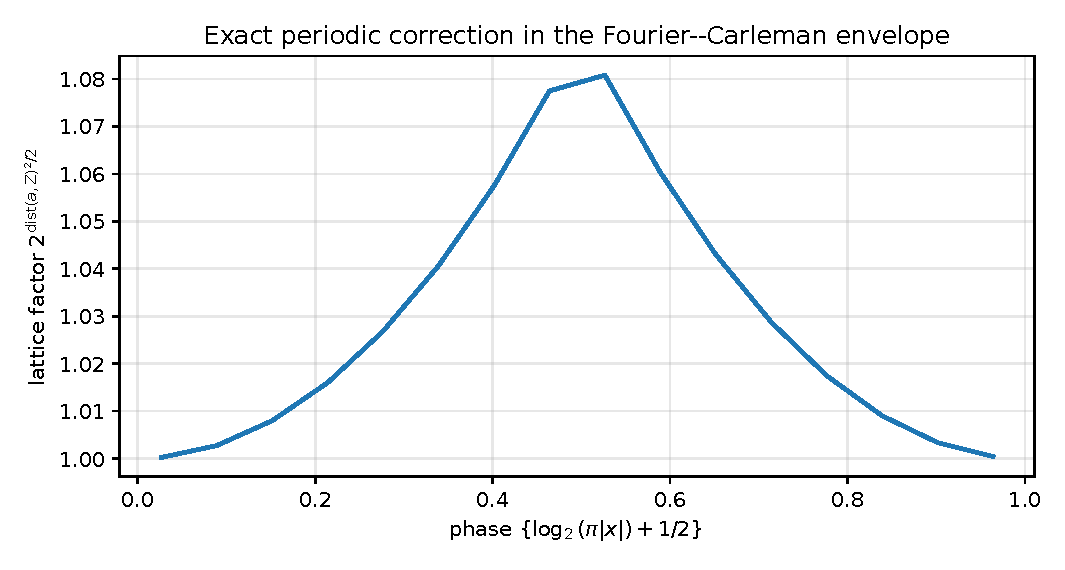
\includegraphics[width=0.88\textwidth]{figures/carleman_lattice_phase.pdf}
  \caption{The exact lattice factor in \eqref{eq:periodic-factor}.  It is not a
  numerical artifact: it is the rounding cost in the discrete Legendre transform.}
  \label{fig:lattice-factor}
\end{figure}

\subsection{What the derivative scale does and does not explain}

The repository's sharp Fourier theorem gives
\begin{equation}
  \AbsoluteValue{\Phi(\xi)}\le C E_{\kappa_\infty}(|\xi|),
  \qquad
  \kappa_\infty=\frac32+\log_2\left(\frac{\pi}{\sqrt3}\right),
  \label{eq:sharp-fourier}
\end{equation}
and proves that no larger algebraic exponent can replace $\kappa_\infty$ globally;
the obstruction occurs on the peak ray
\begin{equation}
  \xi_k=2^k\frac23.
  \label{eq:peak-ray}
\end{equation}
The exact derivative envelope has exponent $\kappa_C$.  Their difference is
\begin{equation}
  \delta=\kappa_\infty-\kappa_C
  =1-\frac12\log_2 3
  =\log_2\left(\frac2{\sqrt3}\right)
  \approx0.2075187496394219.
  \label{eq:delta}
\end{equation}

\begin{theorem}[Exact algebraic gain beyond derivative regularity]
\label{thm:optimal-gain}
There exists $C>0$ such that, for $|\xi|\ge1$,
\begin{equation}
  \AbsoluteValue{\Phi(\xi)}
  \le C B_C(\xi)|\xi|^{-\delta}.
  \label{eq:gain-bound}
\end{equation}
The exponent $\delta$ is optimal: for every $\eta>0$ there is no constant $C_\eta$
with
\begin{equation}
  \AbsoluteValue{\Phi(\xi)}
  \le C_\eta B_C(\xi)|\xi|^{-\delta-\eta}
  \qquad(|\xi|\ge1).
  \label{eq:no-better-gain}
\end{equation}
Indeed, along \eqref{eq:peak-ray},
\begin{equation}
 \frac{\AbsoluteValue{\Phi(\xi_k)}}
 {B_C(\xi_k)\xi_k^{-\delta}}
 =R_*>0
 \qquad(k\ge0),
 \label{eq:constant-peak-ratio}
\end{equation}
with numerically $R_*\approx0.6484307237021603$.
\end{theorem}

\begin{proof}
Since the periodic factor $P$ in \eqref{eq:BC-factor} is bounded above and below,
\eqref{eq:sharp-fourier} is equivalent, up to a constant, to
\eqref{eq:gain-bound}.

For the peak ray, the sinc product factors exactly as
\begin{equation}
 \AbsoluteValue{\Phi(2^k\tfrac23)}
 =\AbsoluteValue{\Phi(\tfrac23)}
 \left(\frac{3\sqrt3}{\pi}\right)^k
 2^{-k(k-1)/2-3k}.
 \label{eq:peak-factorization}
\end{equation}
Moreover $a(\xi_k)=k+a(2/3)$, so the distance $d(\xi_k)$ to the integer lattice is
independent of $k$.  Substitution of \eqref{eq:delta} into
\eqref{eq:BC-closed} shows that the powers of $2$ and the linear powers of $\xi_k$
match exactly, proving \eqref{eq:constant-peak-ratio}.  A bound with
$\delta+\eta$ would force the left side of \eqref{eq:constant-peak-ratio} times
$\xi_k^\eta$ to remain bounded, which is impossible.
\end{proof}

\begin{figure}[htbp]
  \centering
  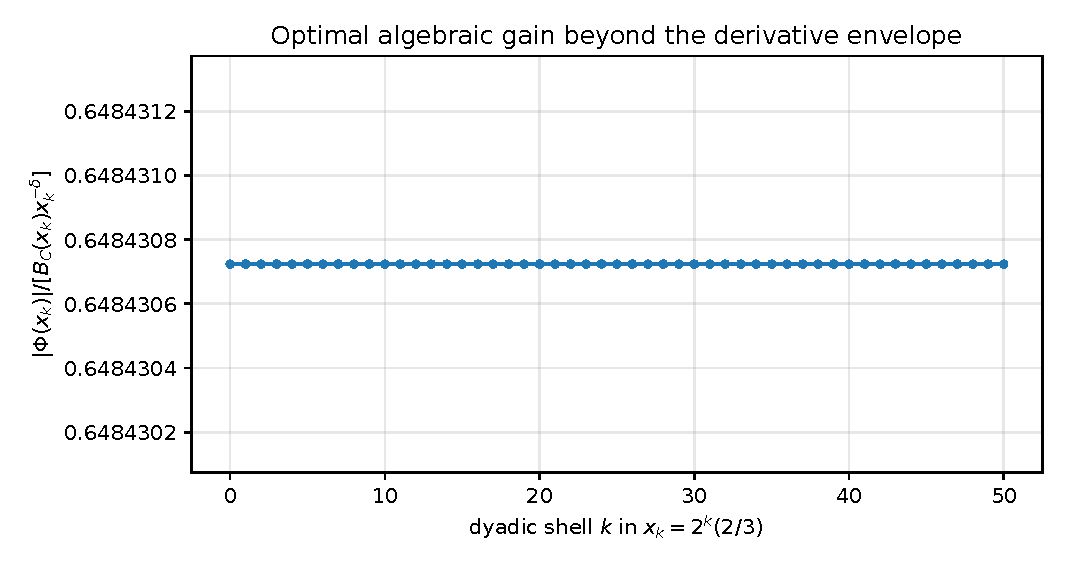
\includegraphics[width=0.88\textwidth]{figures/fourier_optimal_gain_peak_ray.pdf}
  \caption{The normalized peak-ray ratio in \eqref{eq:constant-peak-ratio}.  Its
  phase-locked constancy confirms the exact algebraic gap $\delta$; the plotted
  variation is floating-point roundoff.}
  \label{fig:peak-ratio}
\end{figure}

\begin{remark}[Interpretation]
The quadratic logarithmic Gaussian is already forced by the derivative scale
$W_n$.  The infinite sinc product contributes additional arithmetic information:
the repeated numerator $|\sin(2^m\cdot2\pi/3)|=\sqrt3/2$ along the peak ray yields
exactly $\delta$ further powers.  Thus ultradifferentiable regularity determines the
carrier, while lacunary trigonometric arithmetic determines the sharp algebraic
refinement.
\end{remark}

\section{The associated function and a \texorpdfstring{Lambert--$W_{-1}$}{Lambert-W(-1)} saddle}
\label{sec:associated}

The Fourier envelope above optimizes the \emph{raw} derivative scale after the
$2\pi$ integration-by-parts factor has cancelled one power of $2$ per derivative.
The standard Denjoy--Carleman associated function instead uses the
factorial-normalized sequence $M$:
\begin{equation}
  \omega_M(t)=
  \sup_{n\ge0}\log\left(\frac{t^n}{M_n}\right)
  =\sup_{n\ge0}
  \left(n\log t+\log(n!)-\frac{\log2}{2}n(n+1)\right).
  \label{eq:associated-def}
\end{equation}
The factorial introduces an entropy term $n\log n$, and the optimizer is no longer
an affine function of $\log t$.

\subsection{Continuous saddle and Lambert predictor}

Put $L=\log2$ and extend the objective continuously:
\begin{equation}
  G_t(s)=s\log t+\log\Gamma(s+1)-\frac L2s(s+1),
  \qquad s\ge0.
  \label{eq:Gt}
\end{equation}
Its large saddle $s_t$ satisfies
\begin{equation}
  \log t+\psi(s_t+1)-L\left(s_t+\frac12\right)=0,
  \label{eq:exact-saddle}
\end{equation}
where $\psi=\Gamma'/\Gamma$.
Ignoring the $O(1/s)$ difference between $\psi(s+1)$ and $\log s$ gives the explicit
Lambert predictor
\begin{equation}
  \lambda(t)=
  -\frac1L
  W_{-1}\!\left(-\frac{\sqrt2L}{t}\right).
  \label{eq:lambert-predictor}
\end{equation}
The lower real branch is forced because the relevant saddle tends to infinity.

\begin{theorem}[Lambert saddle and associated-function expansion]
\label{thm:lambert-saddle}
As $t\to\infty$,
\begin{align}
  s_t&=\lambda(t)+O\left(\frac1{\log t}\right),
  \label{eq:s-lambda}\\
  n_*(t)&=s_t+O(1),
  \label{eq:integer-saddle}
\end{align}
where $n_*(t)$ is any integer optimizer in \eqref{eq:associated-def}.  At the
continuous saddle,
\begin{equation}
 G_t(s_t)=
 \frac L2s_t^2-s_t+\frac12\log(2\pi s_t)-\frac12
 +O\left(\frac1{s_t}\right).
 \label{eq:saddle-value}
\end{equation}
Consequently, with $u=\log t$,
\begin{equation}
 \omega_M(t)=
 \frac{u^2}{2L}
 +\frac{u\log u}{L}
 -\left(\frac12+\frac{1+\log L}{L}\right)u
 +O\bigl((\log u)^2\bigr).
 \label{eq:omega-expansion}
\end{equation}
\end{theorem}

\begin{proof}
The expansion
$\psi(s+1)=\log s+1/(2s)+O(s^{-2})$ transforms
\eqref{eq:exact-saddle} into
\[
  Ls-\log s=\log t-\frac L2+O(1/s).
\]
The equation without the error is solved by \eqref{eq:lambert-predictor}.  Its
left derivative is $L-1/s$, bounded away from zero for large $s$, so the saddle
perturbation is $O(1/s)=O(1/\log t)$.  Strict concavity for large $s$ gives
\eqref{eq:integer-saddle}.

At a saddle, substitute
$\log t=L(s+1/2)-\psi(s+1)$ into \eqref{eq:Gt} to obtain
\[
  G_t(s)=\frac L2s^2-s\psi(s+1)+\log\Gamma(s+1).
\]
Stirling expansions of $\log\Gamma$ and $\psi$ yield
\eqref{eq:saddle-value}.  Finally, the Lambert equation gives
\[
  Ls_t=u+\log u-\log L-\frac L2+O\left(\frac{\log u}{u}\right).
\]
Substitution into \eqref{eq:saddle-value}, together with the $O(1)$ rounding loss
from \eqref{eq:integer-saddle}, yields \eqref{eq:omega-expansion}.
\end{proof}

\begin{figure}[htbp]
  \centering
  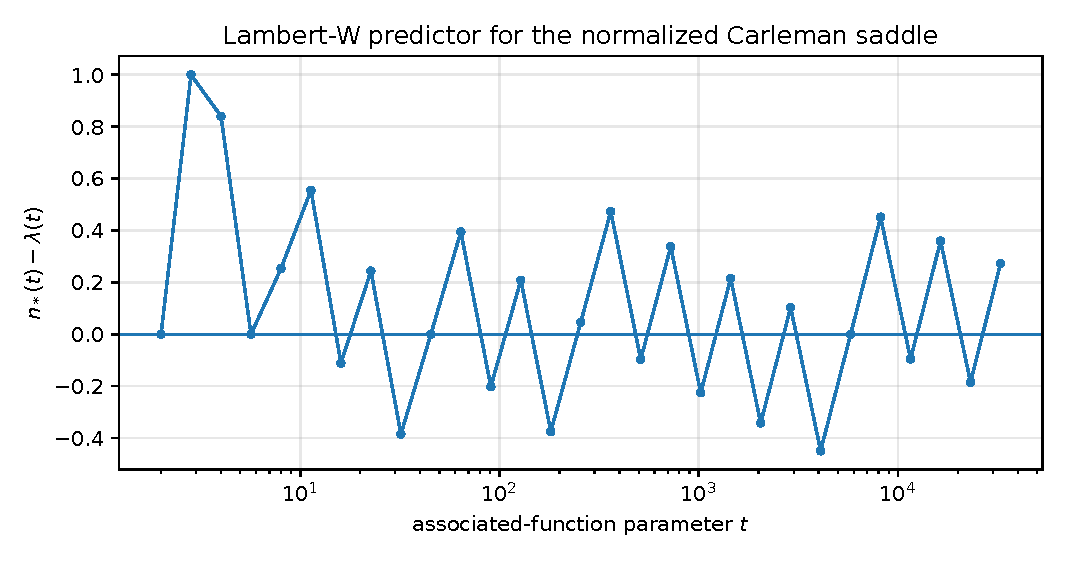
\includegraphics[width=0.88\textwidth]{figures/lambert_saddle_error.pdf}
  \caption{The exact discrete optimizer $n_*(t)$ minus the Lambert predictor
  \eqref{eq:lambert-predictor}.  Integer rounding produces the bounded sawtooth;
  the continuous saddle error is much smaller.}
  \label{fig:lambert-saddle}
\end{figure}

\subsection{Two dualities, two periodic phenomena}

There are now two distinct optimization problems.

\begin{enumerate}[label=(\roman*)]
\item The Fourier integration-by-parts envelope minimizes a pure quadratic over the
integer lattice.  Its optimizer is exactly a rounded affine function of
$\log_2|\xi|$, and its correction is the explicit periodic factor $P(a)$.
\item The standard associated function maximizes a quadratic plus
$\log\Gamma(n+1)$.  The entropy term shifts the saddle by $\log\log t$ and introduces
Lambert $W_{-1}$.  Integer rounding still produces a bounded phase, but now around a
nonlinear Lambert trajectory.
\end{enumerate}

This distinction prevents a common conflation: the Lambert correction is not needed
to optimize the raw Fourier derivative bound, while the exact lattice wave of
\cref{thm:discrete-legendre} is invisible in a purely continuous associated-function
asymptotic.

\section{Geometric-base and \texorpdfstring{$q$}{q}-deformed critical weights}
\label{sec:q-deformation}

The corpus contains geometric-base atomic sinc splines and extensive $q$-analog
machinery.  The regularity scale suggested by those constructions is
\begin{equation}
  W_n^{(b)}=b^{n(n+1)/2},
  \qquad
  M_n^{(b)}=\frac{b^{n(n+1)/2}}{n!},
  \qquad b>1.
  \label{eq:base-b-weight}
\end{equation}
Writing $q=b^{-1}$ makes this
$M_n^{(q)}=q^{-n(n+1)/2}/n!$, the same quadratic exponent that pervades Gaussian
$q$-coefficients.

\begin{theorem}[Base-$b$ weight calculus]
\label{thm:base-b}
Let $b\ge2$ and $L_b=\log b$.  Then:
\begin{enumerate}[label=(\roman*)]
\item
\begin{equation}
  \frac{M_n^{(b)}}{M_{n-1}^{(b)}}=\frac{b^n}{n},
  \label{eq:b-quotient}
\end{equation}
so $M^{(b)}$ is log-convex.
\item
\begin{equation}
 \sum_{k=0}^{\infty}
 \frac{M_k^{(b)}}{(k+1)M_{k+1}^{(b)}}
 =\frac1{b-1},
 \label{eq:b-nqa}
\end{equation}
and
\begin{equation}
 \sum_{j\ge k}\frac{M_{j-1}^{(b)}}{jM_j^{(b)}}
 =\frac{b^{1-k}}{b-1}
 \le\frac{b}{b-1}\frac{M_{k-1}^{(b)}}{M_k^{(b)}}.
 \label{eq:b-strong-nqa}
\end{equation}
\item Moderate growth fails:
\begin{equation}
  \frac{M_{2n}^{(b)}}{(M_n^{(b)})^2}
  =\frac{b^{n^2}}{\binom{2n}{n}}.
  \label{eq:b-moderate}
\end{equation}
\item The Fa\`a di Bruno transform is exact:
\begin{equation}
  \bigl(M^{(b)}\bigr)_n^\circ=b^nM_n^{(b)}.
  \label{eq:b-fdb}
\end{equation}
\item The associated-function saddle has predictor
\begin{equation}
 \lambda_b(t)=
 -\frac1{L_b}
 W_{-1}\!\left(-\frac{\sqrt b\,L_b}{t}\right).
 \label{eq:b-lambert}
\end{equation}
\item The pure quadratic lattice transform satisfies, for $A>1$,
\begin{equation}
 \inf_{n\ge0}\frac{b^{n(n-1)/2}}{A^n}
 =b^{-a_b^2/2+\MetricDistance(a_b,\IntegerNumbers)^2/2},
 \qquad
 a_b=\log_b A+\frac12.
 \label{eq:b-lattice}
\end{equation}
\end{enumerate}
\end{theorem}

\begin{proof}
The quotient, sums, and moderate-growth ratio are direct calculations.
For the Fa\`a di Bruno transform, repeat the proof of
\cref{thm:exact-fdb}.  The factorial ratio is bounded by
$2^{j(r-1)}\le b^{j(r-1)}$, while the all-singleton partition gives the matching
lower bound $(M_1^{(b)})^n=b^n$.  The Lambert and lattice formulas repeat
\cref{thm:lambert-saddle,thm:discrete-legendre} with $\log2$ replaced by $\log b$.
\end{proof}

\begin{remark}[The range $1<b<2$]
The quotient $b^n/n$ is eventually increasing but may fail log-convexity at finitely
many initial indices.  A finite regularization leaves the associated
Denjoy--Carleman class unchanged.  The exact constant in \eqref{eq:b-fdb} can then
change at finitely many orders, while an exponential Fa\`a di Bruno bound and the
same asymptotic Lambert/lattice geometry remain.
\end{remark}

\begin{problem}[Local universality beyond base two]
The binary proof of \cref{thm:local-universality} uses two special facts: an exact
cell profile and uniformly bounded discrepancy of the Thue--Morse signs.  Determine
which base-$b$ atomic spline systems possess a finite-state sign or phase cocycle
with bounded interval discrepancy.  In such systems, prove a local pushforward law
and identify whether its limit is discrete, absolutely continuous, or singular.
\end{problem}

\section{Bell-polynomial edge asymptotics}
\label{sec:bell}

\subsection{The positive critical-norm majorant}

The exact Fa\`a di Bruno transform controls the largest normalized weight of a
single chain-rule partition.  A different object sums all positive Bell terms:
\begin{equation}
  C_n=\frac1{W_n}
  \sum_{k=1}^{n}W_k
  B_{n,k}(W_1,W_2,\ldots,W_{n-k+1}),
  \label{eq:Cn}
\end{equation}
where $B_{n,k}$ is the exponential partial Bell polynomial.  This is the critical
norm majorant one obtains by replacing every derivative amplitude in a self-composition
by its sharp absolute bound and discarding cancellation.  It is deliberately not
identified with an actual derivative of $\FabiusBounded\comp\FabiusBounded$.

The two edges $k\approx n$ and $k\approx1$ dominate, while the middle is suppressed
by the quadratic weight defect.  Several terms can be extracted exactly.

\begin{proposition}[Explicit Bell edges]
\label{prop:bell-edges}
For $n\ge4$, the following contributions to $C_n$ are exact:
\begin{align}
 k=n &: \quad 2^n,
 \label{eq:edge-kn}\\
 k=n-1 &: \quad n(n-1),
 \label{eq:edge-kn1}\\
 k=1 &: \quad 2,
 \label{eq:edge-k1}\\
 k=n-2 &: \quad
 2^{3-n}\left(2\binom n3+3\binom n4\right).
 \label{eq:edge-kn2}
\end{align}
The endpoint split $(1,n-1)$ inside the $k=2$ term contributes exactly
\begin{equation}
  16n\,2^{-n}.
  \label{eq:k2-edge}
\end{equation}
The partition with $k=n-3$ and three blocks of size $2$ contributes exactly
\begin{equation}
  960\binom n6 4^{-n}
  \sim\frac43n^6 4^{-n}.
  \label{eq:three-pairs}
\end{equation}
\end{proposition}

\begin{proof}
For $k=n$, $B_{n,n}=W_1^n$, giving $2^n$.  For $k=n-1$, there is one block of
size $2$ and $n-2$ singletons, so
\[
 \frac{W_{n-1}}{W_n}\binom n2W_2W_1^{n-2}=n(n-1).
\]
The $k=1$ term is $W_1W_n/W_n=2$.

For $k=n-2$, the excess $n-k=2$ is realized either by one $3$-block or two
$2$-blocks.  Their Bell multiplicities are $\binom n3$ and $3\binom n4$, and
substitution of $W_j=2^{T_j}$ gives \eqref{eq:edge-kn2}.

For $k=2$, the two endpoint compositions $(1,n-1)$ combine to
$nW_1W_{n-1}$ inside $B_{n,2}$, yielding \eqref{eq:k2-edge} after multiplication by
$W_2/W_n$.

Finally, three $2$-blocks and $n-6$ singletons have multiplicity
$15\binom n6$.  Their normalized weight is
\[
 \frac{W_{n-3}W_2^3W_1^{n-6}}{W_n}=2^{6-2n}=64\,4^{-n},
\]
which gives \eqref{eq:three-pairs}.
\end{proof}

\subsection{A two-edge asymptotic conjecture}

Define the explicitly subtracted approximation
\begin{equation}
 \begin{split}
 A_n={}&2^n+n(n-1)+2\\
 &+2^{3-n}\left(2\binom n3+3\binom n4\right)
 +16n\,2^{-n}.
 \end{split}
 \label{eq:An}
\end{equation}
All values in the accompanying computation are exact rational numbers until the
final decimal output.

\begin{conjecture}[First unremoved Bell edge]
\label{conj:bell-four-thirds}
As $n\to\infty$,
\begin{equation}
  C_n-A_n
  \sim\frac43n^6 4^{-n}.
  \label{eq:bell-conj}
\end{equation}
Equivalently,
\begin{equation}
  \lim_{n\to\infty}
  \frac{4^n}{n^6}(C_n-A_n)=\frac43.
  \label{eq:bell-limit}
\end{equation}
\end{conjecture}

The candidate constant is not curve fitting: it is forced by the three-pair term
\eqref{eq:three-pairs}.  Other $k=n-3$ block patterns have lower polynomial degree,
while the $k=3$ left edge is of order $n^2 4^{-n}$.  Terms farther from either edge
carry an additional exponential defect.  A proof should convert this heuristic into
a uniform two-edge tail estimate.

\begin{table}[htbp]
\centering
\caption{Exact-arithmetic evidence for \cref{conj:bell-four-thirds}.}
\label{tab:bell-data}
\begin{tabular}{rr}
\toprule
$n$ & $4^n(C_n-A_n)/n^6$ \\
\midrule
20  & 0.932702130656337 \\
40  & 1.116793440375664 \\
60  & 1.185331851851859 \\
80  & 1.220944228515625 \\
100 & 1.242749164800000 \\
120 & 1.257470214763374 \\
\bottomrule
\end{tabular}
\end{table}

\begin{figure}[htbp]
  \centering
  \begin{subfigure}[t]{0.48\textwidth}
    \centering
    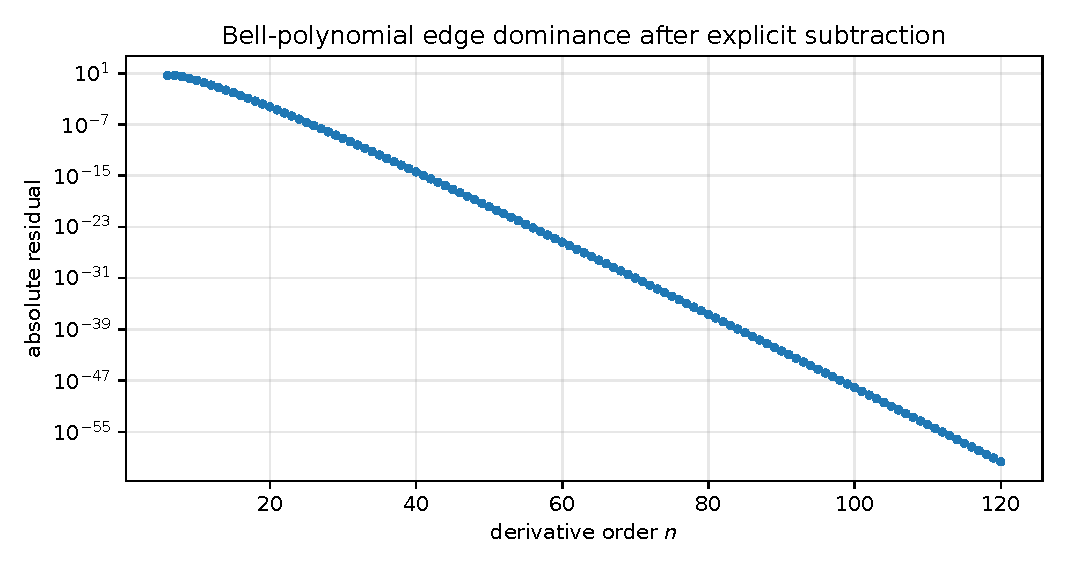
\includegraphics[width=\textwidth]{figures/bell_edge_residual.pdf}
    \caption{Unscaled residual.}
  \end{subfigure}\hfill
  \begin{subfigure}[t]{0.48\textwidth}
    \centering
    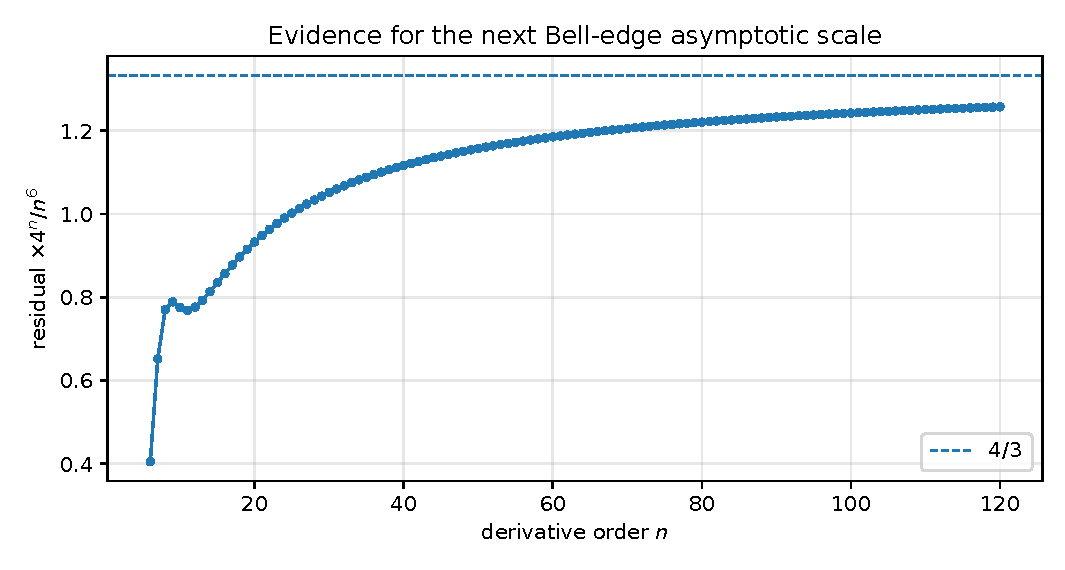
\includegraphics[width=\textwidth]{figures/bell_edge_scaled_residual.pdf}
    \caption{Scaled residual and the conjectural $4/3$ limit.}
  \end{subfigure}
  \caption{Two-edge Bell-polynomial numerics through $n=120$.}
  \label{fig:bell}
\end{figure}

\begin{conjecture}[Full Bell-edge transseries]
\label{conj:bell-transseries}
The sequence $C_n$ has an asymptotic expansion organized by distance from the two
Fa\`a di Bruno edges.  For fixed right defect $d=n-k$, the leading term comes from
$d$ two-blocks and has the form
\begin{equation}
  \frac{(2d)!}{2^d d!}\binom n{2d}
  2^{d(d+1)/2-(d-1)n}.
  \label{eq:right-edge-general}
\end{equation}
For fixed left order $k$, the leading term comes from one block of size $n-k+1$ and
$k-1$ singletons.  After subtracting finitely many terms from both edges, the
remaining middle is exponentially smaller than the first omitted edge scale.
\end{conjecture}

This conjecture would turn the positive Bell majorant into a precise asymptotic
counterpart of the signed partition-defect theory in \cite{ProveItIterates}.  It may
also supply a reusable template for base-$b$ and $q$-Bell compositions.

\section{Further conjectures and a research program}
\label{sec:future}

\subsection{Microlocal and Fourier questions}

\begin{problem}[Fourier characterization at the critical weight]
Develop a Paley--Wiener or almost-holomorphic characterization tailored to
$M_n=2^{T_n}/n!$ that retains the exact lattice phase of
\cref{thm:discrete-legendre}.  Standard equivalence up to exponential constants
forgets the factor $P(a)$; the goal is a phase-sensitive refinement that recovers it
from complex extension or short-time Fourier data.
\end{problem}

\begin{conjecture}[A periodic ultradifferentiable wavefront profile]
For compactly supported functions saturating the critical derivative sequence, the
optimal logarithmic-Gaussian Fourier carrier admits a bounded one-periodic profile
in $\log_2|\xi|$.  For $\RvachevUp$, the derivative-lattice profile $P$ and the sinc-product
arithmetic profile combine multiplicatively, with the peak ray selecting a fixed
phase.
\end{conjecture}

\subsection{Inverse endpoints and two-regime regularity}

\begin{problem}[Interior critical class versus endpoint transseries]
Match the interior class $\Roumieu{M}\setminus\Beurling{M}$ of
$\FabiusQuantile=\FabiusBounded^{-1}$ to the
known Lambert--periodic endpoint expansion as $y\downarrow0$.  A satisfactory
connection should identify a scale-dependent crossover: derivatives on compact
interior intervals are governed by $M$, while the shrinking endpoint neighborhood
introduces the Lambert saddle and periodic endpoint phase.
\end{problem}

\begin{conjecture}[Endpoint-rescaled Carleman type]
There exists a two-parameter asymptotic for
$\sup_{y\in[\eta,2\eta]}|\FabiusQuantile^{(n)}(y)|$ in the joint limit $n\to\infty$,
$\eta\downarrow0$, whose transition curve is expressed through the same
$W_{-1}$ phase that governs the endpoint inverse expansion.  Away from that curve
it reduces either to an $M_n$-type interior bound or to the endpoint transseries.
\end{conjecture}

\subsection{Extension theory without moderate growth}

The exact weight is strongly nonquasianalytic but not moderate.  This places it
between two familiar regimes: compactly supported functions and nonlinear calculus
are available, while several standard Whitney-extension and tensor-product theorems
cannot be invoked automatically.

\begin{problem}[Optimal descendant and Whitney extension]
Construct the optimal descendant weight associated with $M$ and determine whether
Whitney jets on intervals or tame closed sets admit extension without loss, with a
finite loss, or only through a weight matrix.  Express any loss in the Lambert
associated-function scale \eqref{eq:omega-expansion}.
\end{problem}

\subsection{\texorpdfstring{$q$}{q}, cyclotomic, and arithmetic deformations}

\begin{problem}[Cyclotomic Carleman geometry]
For complex $q$ approaching a root of unity, combine the branch geometry of the
corpus's inverse $q$-analogs with the quadratic weight
$q^{-T_n}/n!$.  Determine how the associated Lambert saddle bifurcates when
$\log q$ becomes multivalued and whether the lattice correction becomes a
higher-dimensional torus phase.
\end{problem}

\begin{conjecture}[Base-deformed exact type]
For every geometric atomic spline in the corpus whose derivatives have exact
$L^1$ scale $b^{T_n}$, the sharp Fourier envelope decomposes into
\[
 \text{base-$b$ quadratic carrier}
 \times\text{integer-lattice phase}
 \times\text{arithmetic gain}.
\]
The first two factors are universal consequences of the critical weight; the third
is determined by the extremal orbit of the base-$b$ trigonometric numerator.
\end{conjecture}

\subsection{Formalization roadmap}

The following sequence is designed to minimize dependencies.

\begin{enumerate}[label=\textbf{L\arabic*.},leftmargin=2.5em]
\item Formalize $P(2m)=0$, $P(2m+1)=\ThueMorseSign{m}$, and block discrepancy
      at most $2$.
\item Combine the existing exact cell identity with interval-cell decomposition to
formalize \cref{thm:local-universality} first for simple functions $H$, then for
bounded Borel tests or, more modestly, continuous tests.
\item Formalize the eventual local extrema theorem, which needs only three complete
cells and the no-three-equal-sign lemma.
\item Define interval Roumieu/Beurling seminorms and prove the sequence-comparison
criterion \cref{thm:dc-classification}.
\item Formalize the quotient identities, nonquasianalytic sums, and failure of
moderate growth.
\item Define the Fa\`a di Bruno sequence transform and prove
$M_n^\circ=2^nM_n$ using the one-large-part reduction.
\item Import the existing iterate spine theorem and derive the exact critical class
of all forward and inverse iterates.
\item Formalize the integer quadratic optimizer and lattice factor in
\cref{thm:discrete-legendre}; this is independent of analytic Fourier machinery.
\item Formalize the Lambert predictor only after a reusable real $W_{-1}$ asymptotic
library is in place.
\item Treat the Bell-edge conjecture last; exact recurrences and finite certificates
can be formalized before the asymptotic tail estimate.
\end{enumerate}

\section{Reproducible numerical experiments}
\label{sec:numerics}

No numerical computation is used to prove the local universality theorem, the exact
Denjoy--Carleman classification, the weight geometry, the Fa\`a di Bruno transform,
the iterate synthesis, or the Fourier lattice formula.  The script
\path{frontier_experiments.py} has four narrower purposes:

\begin{enumerate}[label=(\roman*)]
\item verify the direct integer infimum and the closed form
\eqref{eq:BC-closed} over a logarithmic frequency grid;
\item evaluate the exact peak-ray factorization and the normalized constant in
\eqref{eq:constant-peak-ratio};
\item compare the exact integer optimizer of $\omega_M$ with the Lambert predictor;
\item compute $C_n$ by exact integer Bell recurrences through $n=120$ and test
\cref{conj:bell-four-thirds}.
\end{enumerate}

The command is
\begin{lstlisting}[language=bash]
python3 frontier_experiments.py --out-dir .
\end{lstlisting}
The dependencies are Python $3$, \texttt{mpmath}, and \texttt{matplotlib}.  CSV
outputs preserve long decimal strings; Bell-polynomial arithmetic uses Python
integers and \texttt{fractions.Fraction} until serialization.  Both vector PDF and
PNG figures are generated.  The archive includes the script, requirements file,
all CSV tables, figures, a numerical summary, and a SHA-256 ledger.

\begin{table}[htbp]
\centering
\caption{Numerical constants independently reproduced by the script.}
\label{tab:constants}
\begin{tabular}{ll}
\toprule
Quantity & Value \\
\midrule
$\Phi(2/3)$ & $0.3216018886465493980463579415952921\ldots$ \\
$\kappa_C$ & $2.1514961294723187980432792951080073\ldots$ \\
$\kappa_\infty$ & $2.3590148791117407073164098231340991\ldots$ \\
$\delta$ & $0.2075187496394219092731305280260917\ldots$ \\
$R_*$ & $0.6484307237021602497560540918702998\ldots$ \\
\bottomrule
\end{tabular}
\end{table}

\section{Conclusions}
\label{sec:conclusion}

The dyadic derivative factor $2^{n(n+1)/2}$ is more than a convenient upper bound.
It is a complete local regularity invariant.

The exact cells and bounded Thue--Morse discrepancy force every interval to sample
the same normalized derivative law.  That local law upgrades a global sharp bound
to exact local extrema, moment limits, and a complete comparison theorem against
all Denjoy--Carleman sequences.  Factorial normalization then reveals a critical
weight that is simultaneously nonquasianalytic, nonmoderate, and closed under the
nonlinear operations central to the Fabius system.  Its exact Fa\`a di Bruno
transform makes the closure quantitative.

The same scale also clarifies two apparently different parts of the corpus.  On the
dynamical side, it converts the existing dominant-spine lower bounds into an exact
Roumieu-versus-Beurling classification for every forward and inverse iterate.  On
the Fourier side, it supplies the logarithmic-Gaussian carrier, while the sinc
arithmetic contributes an exactly measurable extra algebraic gain.  The discrete
integer optimizer leaves a periodic lattice fingerprint; the factorial-normalized
associated function instead introduces Lambert $W_{-1}$ through its entropy-shifted
saddle.

This regularity layer is compatible with, but not a duplication of, the corpus's
$q$-analog, Lambert, Fourier, inverse, Legendre, Bell--Bernoulli, and representation
programs.  It provides a common scale on which those programs can interact.  The
most immediate next targets are the uniform iterate type formula, a phase-sensitive
Fourier characterization, a rigorous Bell-edge transseries, and a base-$b$ local
universality theorem.

\appendix

\section{Additional proof details}
\label{app:details}

\subsection{Why the one-large-part product is maximal}

For completeness, suppose $M$ is log-convex, so its quotients
$\mu_n=M_n/M_{n-1}$ are increasing.  If $2\le a\le b$, then
\[
 \frac{M_{a-1}M_{b+1}}{M_aM_b}
 =\frac{\mu_{b+1}}{\mu_a}\ge1.
\]
Thus transferring one unit from a smaller part $a$ to a larger part $b$ does not
decrease the product.  Iterating pushes every composition
$\alpha_1+\cdots+\alpha_j=n$ to $(n-j+1,1,\ldots,1)$ and proves the reduction used
in \cref{thm:exact-fdb}.

\subsection{Right-edge Bell exponents}

Let $k=n-d$ and write the block sizes as $\alpha_i=1+\beta_i$, with
$\beta_i\ge0$ and $\sum_i\beta_i=d$.  The normalized base-$2$ exponent of the
corresponding Bell weight is
\begin{equation}
 E(d,\boldsymbol\beta)
 =T_{n-d}+\sum_iT_{1+\beta_i}-T_n
 =-(d-1)n+\frac{d^2+\sum_i\beta_i^2}{2}.
 \label{eq:right-edge-exponent}
\end{equation}
For fixed $d$, the largest polynomial multiplicity occurs when all positive
$\beta_i$ equal $1$, i.e. when there are $d$ two-blocks.  There are
\[
  \frac{(2d)!}{2^d d!}\binom n{2d}
\]
such set partitions, and their exponent is
$d(d+1)/2-(d-1)n$, giving \eqref{eq:right-edge-general}.  This calculation explains
both the exact $d=3$ candidate and the expected hierarchy in
\cref{conj:bell-transseries}.

\subsection{The peak-ray constant}

Let
\[
  a_0=\log_2(2\pi/3)+\frac12,
  \qquad d_0=\MetricDistance(a_0,\IntegerNumbers).
\]
Then \eqref{eq:constant-peak-ratio} has the explicit value
\begin{equation}
  R_*=\AbsoluteValue{\Phi(2/3)}
  \left(\frac23\right)^\delta
  2^{a_0^2/2-d_0^2/2}.
  \label{eq:Rstar}
\end{equation}
The equality for all $k$ is exact; the numerical script evaluates
$\Phi(2/3)$ by a high-precision tail-controlled sinc product.

\section{Artifact inventory and reproducibility}
\label{app:artifact}

The accompanying archive has the following layout.

\begin{center}
\begin{tabularx}{0.94\textwidth}{>{\ttfamily\raggedright\arraybackslash}p{0.38\textwidth}X}
\toprule
Path & Purpose \\
\midrule
fabius\_carleman\_frontiers.tex & Complete LaTeX source. \\
fabius\_carleman\_frontiers.pdf & Rendered report. \\
frontier\_experiments.py & Commented deterministic numerical experiment. \\
requirements.txt & Minimum Python dependencies. \\
README.txt & Build and reproduction instructions. \\
numerical\_summary.txt & Key constants and run scope. \\
data/*.csv & Gauge, peak-ray, Lambert-saddle, and Bell data. \\
figures/*.pdf & Vector figures used by the report. \\
figures/*.png & Raster inspection copies. \\
CORPUS\_AUDIT.txt & Scope and novelty-screen record. \\
SHA256SUMS.txt & Checksums for all archive payloads. \\
\bottomrule
\end{tabularx}
\end{center}

The PDF was built with \texttt{latexmk}, rendered page-by-page for visual
inspection, and checked for structural and font issues.  The numerical script is
not network-dependent.

\begingroup
\small
\begin{thebibliography}{99}

\bibitem{AriasFabius}
J. Arias de Reyna,
\newblock Arithmetic of the Fabius function,
\newblock \emph{Integers} \textbf{18} (2018), Article A51, 20 pp.;
\newblock arXiv:1702.06487.

\bibitem{RainerSchindl}
A. Rainer and G. Schindl,
\newblock Equivalence of stability properties for ultradifferentiable function
classes,
\newblock \emph{Rev. R. Acad. Cienc. Exactas F\'{\i}s. Nat. Ser. A Mat. RACSAM}
\textbf{110} (2016), 17--32,
\newblock doi:10.1007/s13398-014-0216-0.

\bibitem{RainerComposition}
A. Rainer and G. Schindl,
\newblock Composition in ultradifferentiable classes,
\newblock \emph{Studia Math.} \textbf{224} (2014), 97--131,
\newblock doi:10.4064/sm224-2-1.

\bibitem{RainerClosedSets}
A. Rainer,
\newblock Arc-smooth functions on closed sets,
\newblock \emph{Compos. Math.} \textbf{155} (2019), 645--680,
\newblock arXiv:1801.08335.

\bibitem{ProveItDocs}
V. Reshetnikov,
\newblock \emph{ProveIt: Analysis/FabiusFunction/docs}, live documentation tree,
\newblock \url{https://github.com/VladimirReshetnikov/ProveIt/tree/main/Analysis/FabiusFunction/docs},
\newblock accessed 30 August 2026.

\bibitem{ProveItMain}
V. Reshetnikov,
\newblock \emph{Fabius Function and Rvachev Up}, canonical LaTeX exposition,
\newblock \url{https://github.com/VladimirReshetnikov/ProveIt/blob/main/Analysis/FabiusFunction/docs/Fabius_Function_and_Rvachev_Up/Fabius_Function_and_Rvachev_Up.tex},
\newblock accessed 30 August 2026.

\bibitem{ProveItFrontier}
V. Reshetnikov,
\newblock \emph{Semi-formalized Research Frontiers}, canonical LaTeX volume,
\newblock \url{https://github.com/VladimirReshetnikov/ProveIt/blob/main/Analysis/FabiusFunction/docs/semi-formalized-research-frontiers/semi-formalized-research-frontiers.tex},
\newblock accessed 30 August 2026.

\bibitem{ProveItManifest}
V. Reshetnikov,
\newblock \emph{Draft Manifest}, global thematic inventory and provenance map,
\newblock \url{https://github.com/VladimirReshetnikov/ProveIt/blob/main/Analysis/FabiusFunction/docs/semi-formalized-research-frontiers/drafts/MANIFEST.md},
\newblock accessed 30 August 2026.

\bibitem{ProveItArchive}
V. Reshetnikov,
\newblock \emph{Archive of Historical Document Versions},
\newblock \url{https://github.com/VladimirReshetnikov/ProveIt/tree/main/Analysis/FabiusFunction/docs/archive},
\newblock accessed 30 August 2026.

\bibitem{ProveItIterates}
V. Reshetnikov,
\newblock \emph{Nowhere Analyticity of Every Positive Compositional Iterate of the
Fabius Function: A Dyadic-Spine Proof through Fa\`a di Bruno Partitions},
\newblock \url{https://github.com/VladimirReshetnikov/ProveIt/blob/main/Analysis/FabiusFunction/docs/semi-formalized-research-frontiers/drafts/representations/fabius_iterates_nowhere_analytic/fabius_iterates_nowhere_analytic.tex},
\newblock 30 August 2026.

\end{thebibliography}
\endgroup

\end{document}
